\section{Conclaves Summary}
\label{sec:conclaves-summary}

I designed and implemented \emph{conclaves}~\cite{phoenix-conclaves}---a
container of enclaves---as a solution for a party to run multi-process
applications that compute with sensitive data on an untrusted third-party
machine.
%
As a motivating use case, I focus on a content provider using a CDN to serve
their HTTPS website; the CDN's webservers run in a conclave, thereby guarding
the content provider's private TLS key, the TLS session keys, and optionally
the content itself, essentially reducing the adversarial power of the CDN to
that of an on-path TLS attacker.

\subsection{Design and Implementation}

% Design diagram {{{

\begin{figure}
\centering
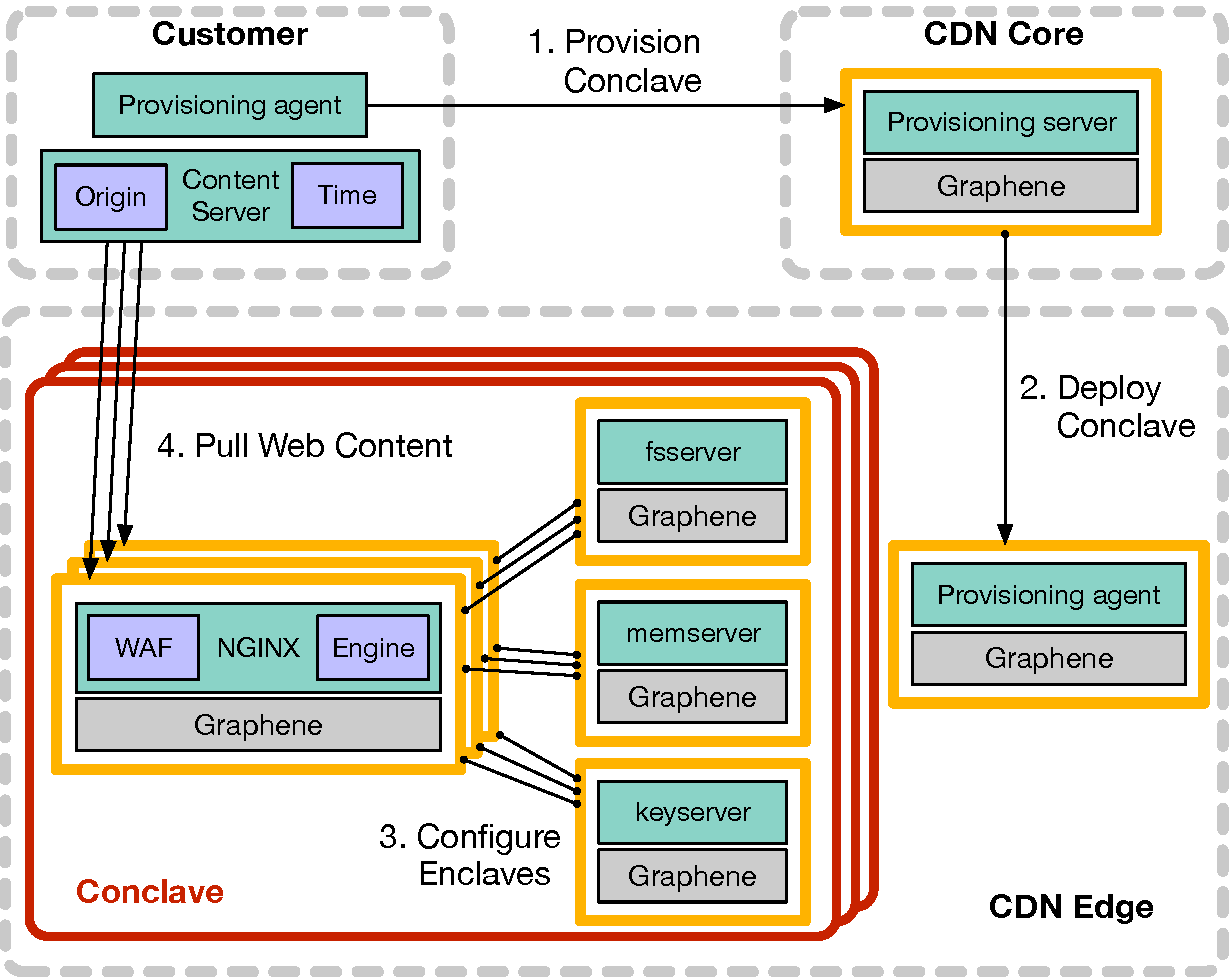
\includegraphics[width=0.48\textwidth]{figs/phoenix-design}
	\caption{Architectural design of a CDN webserver using conclaves. Multiple enclaves (yellow
	boxes) reside in a logical conclave (red boxes), permitting
	multiple processes and multi-tenant deployments. The CDN Edge and
	Core servers run on untrusted hosts.}
\label{fig:design}
\end{figure}

% }}}

The conclave design extends the open-source Graphene SGX libOS~\cite{graphene}
to support shared state abstractions among multiple processes.
%
Graphene~\cite{graphene} supports the critical system calls
\texttt{fork} and \texttt{exec} by automatically spawning a brand new
enclave, and performing a checkpoint-and-migration (essentially copying
the first enclave's memory pages into the second).
%
Graphene further offers some support for these separate processes
(enclaves) to communicate with one another over pipes, and implements
copy-on-write fork, signals, semaphores, message queues, and exit
notifications as RPCs over these pipes.
%
In other words, Graphene essentially turns a traditional multi-process
application into a ``distributed system'' of enclaves, along with some
basic plumbing to allow them to communicate with one another.


%% Key design challenges for libOSes include support for \texttt{fork} and
%% \texttt{exec}, and the subsequent management of shared state among the
%% processes.
%% %
%% Of the SGX-based libOSes, only Graphene supports forking, which it models as a
%% checkpoint and restore process migration.
%% %
%% In Graphene, multiple libOS instances coordinate over pipes to implement a
%% consistent, distributed POSIX abstraction, yet appear to the application as a
%% single, shared OS\@.  
%% %
%% In particular, Graphene implements copy-on-write fork, signals, semaphores,
%% message queues, and exit notifications as remote procedure calls (RPCs) over
%% these pipes.

However, two important multi-process abstractions that Graphene does not support with
confidentiality and integrity guarantees are a read-write filesystem, and
shared memory.
%
Graphene's sole filesystem, \texttt{chrootfs}, is modeled as a restricted view
of the host's filesystem.
%
%The contents of the filesystem are in plaintext; for read-only files, Graphene
%ensures the integrity of the file's contents by loading cryptographic hashes
%of the content into the enclaved libOS and verifying these hashes upon file
%reads; writable files have no integrity protections.
%
Graphene does not support shared memory at all (neither anonymous nor
file-backed).


Conclaves extend upon this prior design by leaning into the distributed
system nature of it.
%
I implement kernel services as \emph{kernel servers}; applications
act as clients, connecting to and issuing requests to kernel
services---via pipes or TLS network connections.
%
The kernel servers also run atop the libOS.
%
My design is effectively that of a multi-server microkernel system,
similar to GNU Hurd or Mach-US, in which shared resource abstractions
are implemented as a set of enclaved daemons shared by all processes in
the system.
%% The daemons themselves also run atop the libOS\@.


\subsubsection{Conclave Kernel Servers}

Using the NGINX web server as a guide (as software representative of a
CDN edge server), I identified five key shared resources: files,
shared memory, locks/semaphores, cryptographic keys, and time.  
%
For flexibility in deployment configurations, I implement four servers
to manage these resources\footnote{Due to the common pattern of using
locks with shared memory, the memserver manages both.}:
%
I implement the fsserver, memserver, and keyserver as single-threaded,
single-process, event-driven servers that communicate with the application's
Graphene instances over a TLS-encrypted stream channel. 
%
The timeserver uses a datagram channel.
%
Each server is independent.


\parhead{fsserver}
%
For my file server, \emph{nextfs}, I extend lwext4's~\cite{lwext4} userspace
implementation of an ext2 filesystem into a networked server.
%
nextfs uses an untrusted host file as the backing store, similar to a block
device.
%
I develop three variants of this device to accommodate different security
postures, and a fourth for comparison purposes.

\vspace*{-0.5\baselineskip}
\begin{widelist}

\item 
%
\textbf{bd-std} stores data blocks in plaintext, without integrity
guarantees. This serves as a baseline in my evaluation.


\item
%
\textbf{bd-crypt} encrypts each block using AES-256 in XTS mode, the de
	facto standard for full-disk encryption~\cite{xts-ieee,xts-nist}.
%
I base each block's initialization vector on the block's ID.
%
This, too, lacks integrity guarantees, and is thus suitable only for an
	honest-but-curious attacker.


\item
%
\textbf{bd-vericrypt} adds integrity guarantees to bd-crypt, thus
	providing authenticated encryption.  It does so by maintaining a
	Merkle tree over the blocks: a leaf of the tree is an HMAC of the
	associated (encrypted) block, and an internal node the HMAC of its
	two children.
%
To keep the memory needs of the enclave small, bd-verity consults a
	serialized representation of the tree in a separate file, rather
	than use an in-memory representation.
%
The root of the Merkle tree exists both on the file and in enclave
	memory; the HMAC key exists only in enclave memory.
%
As an optimization for reducing reads and writes to the Merkle tree
	file, bd-verity maintains an in-enclave LRU-cache of the tree
	nodes.
	%
	bd-vericrypt is the appropriate choice in a Byzantine threat model.
	

\end{widelist}


\parhead{memserver}
%
I implement shared memory as filesystems that implement a
reduced set of the filesystem API\footnote{Graphene does not have a
unified filesystem and memory subsystem, and
thus \texttt{munmap} is not currently available as a filesystem operation.
}:
\texttt{open}, \texttt{close}, \texttt{mmap}, and \texttt{advlock}
(\texttt{advlock} handles both advisory locking and unlocking).
%
In my shared memory filesystems, files are called \emph{memory files}, and
either represent a pure, content-less lock, or a lock with an associated
shared memory segment.
% 
Memory files are non-persistent: they are created on the first open and
destroyed when no process holds a descriptor to the file and no process has the
associated memory segment mapped.


I implement three versions of shared memory.
%
Each stores a canonical replica of the shared memory at a known
location (either a particular server or file).
%% Each uses a scheme whereby a canonical replica of the shared memory is
%% stored at a known location.  
%
Upon locking a file, the client ``downloads" the canonical replica and updates
its internal memory maps.
%
On unlock, the client copies its replica to the canonical.
%
%Note that SGX does not provides a means for us to interpose on page accesses
%(as a page table handler would in normal Linux), and thus we must 
%interpose through the locking and unlocking system calls.
%\begin{widelist}

\vspace*{-0.5\baselineskip}
\begin{widelist}

\item 
%
\textbf{sm-vericrypt-basic} uses an enclaved server to keep the canonical
memory files in an in-enclave red-black tree.

\item 
% 
\textbf{sm-vericrypt} implements a memory file as two untrusted host files: a
mandatory lock file, and an optional segment file.
%
When a client opens a memory file, the sm-vericrypt server creates the lock file on the
untrusted host, and the Graphene client maps (\texttt{MAP\_FILE|MAP\_SHARED})
the lock file into untrusted memory.
%
The client then constructs a ticketlock structure over this untrusted shared
memory.
%
Since the untrusted host may manipulate the ticketlock's turn value, a
shadowed, trusted turn number is maintained by the enclaved sm-vericrypt
server.
%
After the client has acquired the lock, the client makes an RPC to the
server to verify the turn number.
%
The server thus acts as a trusted monitor of the untrusted monotonic
	counter.
%% As such, the server acts as a trusted, monotonic counter that monitors an
%% untrusted monotonic counter.


If a client \texttt{mmap}s the memory file, the server creates the
associated segment file on the untrusted host.
%
When the client subsequently locks the file, the client makes a \texttt{lock}
RPC to server, which returns the keying and MAC tag information for
the segment.
%
The client copies the untrusted memory segment into the enclave, and uses
AES-256-GCM to decrypt and authenticate the data.
% 
When a client unlocks the file, the client generates a new IV, copies an
encrypted version of its in-enclave memory segment into the untrusted
segment file, and makes an \texttt{unlock} RPC to the server, passing along
the new IV and MAC tag.

% \clg{I think this section can be compressed}

\item 
%    
\textbf{sm-crypt} 
	%is like sm-vericrypt, but 
	assumes the untrusted host does not
tamper with data.  As such, sm-crypt uses AES-256-CTR instead of AES-256-GCM,
and does not need an enclaved server to monitor the integrity of the ticketlock
and IV.

\end{widelist}


\parhead{keyserver}
%
The keyserver is an SGX enclave rendition of a hardware-security module
(HSM): the keyserver stores private keys and performs any private key
cryptographic operations.
%
Like Keyless SSL~\cite{keyless-ssl}, this not only maintains the
confidentiality of the private key with respect to an untrusted host,
but also isolates the key to an address space distinct from the
application's, thereby guarding against critical memory disclosure
vulnerabilities, such as Heartbleed~\cite{heartbleed-cve}.


I implement the keyserver as two components: the keyserver proper, and an
OpenSSL engine (``engine'' in Figure~\ref{fig:design}) that the application
loads as a shared library; the engine proxies private key operations to the
keyserver.
%
Unlike the fsserver and memserver clients, the key client operates at
the application layer, outside of Graphene.


OpenSSL's engine API requires the caller (in my case, NGINX) to provide an
\texttt{RSA} object, which contains the secret key.
%
To avoid having to expose the key, I modified OpenSSL to populate
\texttt{RSA} objects with dummy keys that instead serve as identifiers
that the keyserver uses to look up the real keys it stores securely.


To reduce the number of connections and avoid a dependency on the memserver for
lock files, my engine maintains the property that all keys for the same
keyserver, within the same process, share a single connection.
%
This requires that the engine detect forking by the application, which we
achieve by also associating process IDs with the \texttt{RSA} objects.


\parhead{timeserver}
%
Given that the components of a conclave must authenticate one another,
I need trusted time to guard against attacks that 
% manipulate the conclave's sense of time to
trick the conclave into accepting expired certificates.
%% (and therefore possibly
%% cracked) certificates.
%
Unfortunately, SGX itself does not provide trusted time.  
%
Its SDK~\cite{sgx-linux-sdk} provides features~\cite{sgx-trusted-time}
for retrieving coarse-grained, monotonic time through a protected clock
provided by Intel's Converged Security and Management Engine (CSME),
but not all processors support it~\cite{ayeks-sgx-hardware}.
%

%% Techniques that base wall-clock time on the \texttt{RDTSC} family of x86
%% instructions cause a \texttt{\#UD} fault in SGXv1, while in SGXv2 the
%% instruction may be modified by a hypervisor.
%% %
%% Intel's SGX SDK~\cite{sgx-linux-sdk} does provide
%% features~\cite{sgx-trusted-time} for retrieval of coarse grained, monotonic
%% time, through a protected clock provided by Intel's Converged Security and
%% Management Engine (CSME)\@.  
%% %
%% However, this feature relies on the presence of the CSME (not all processors
%% include this firmware~\cite{ayeks-sgx-hardware}), and moreover relies on an
%% enclave to securely obtain a base wall-clock time from a remote, trusted,
%% server.


Instead of relying on the CSME, I simply design a remote, signed
timestamping server.
%
The timestamping server runs outside of an enclave, on a remote trusted
machine (e.g., at the CDN's customer).
%
The timeserver's purpose is not to provide fine grained precision to
the conclaved processes, but rather to serve as an integrity check of
the time those processes receive from the untrusted host.

I modify the Graphene system call handlers for \texttt{getttimeofday},
\texttt{time}, and \texttt{clock\_gettime} to optionally proxy application
calls to a remote, trusted, timestamp signing server.
%
The use of such a timeserver, and the related parameters, such as the
timeserver's public key, are specified by the Graphene user (here, the content
provider), and hard-coded into Graphene's configuration.
%
As a freshness guarantee, each request includes a new, random
nonce, generated by the Graphene system call handlers.
%
The timeserver, in turn, returns an RSA signature over a message
consisting of the current time concatenated with this nonce.


%% As time-related system calls occur frequently in event-driven applications like
%% web servers, and as each timeserver request incurs latency due to both the
%% network and RSA operations, the Graphene client makes remote requests for  $p$
%% percent of the time-related system calls, where $p$ is a configurable
%% parameter.
%% %
%% Upon verifying a timeserver response, the Graphene client retrieves the time
%% as reported by the untrusted host, and verifies that the time the host
%% returns is within a configurable tolerance to the timeserver's time.
%% %
%% For a time-related call in which the Graphene client does not consult the
%% timeserver, Graphene checks that the time returned by the untrusted host is
%% greater than the last time value retrieved.


My timeserver approach resembles Google's roughtime protocol~\cite{roughtime};
future work would fully port the roughtime protocol to Graphene to reduce the
need for a trusted timeserver by instead tolerating some fraction of
misbehaving servers.
%
Note, however, that, in the SGX setting, both my approach and roughtime are best
efforts; an untrusted host that identifies the traffic between the Graphene
client and timeserver could, for instance, ``slow down" time by delaying the
responses.



\subsubsection{Conclave Images} % {{{

Conclaves bundle the SGX microkernel runtime and application suite into a
deployable and executable image, reminiscent of a traditional container image.
%
When the conclave is executed, the first enclave process that is
executed is an init process, which executes the kernel servers and the
specified application proper.
%
From that point, the application can fork, spin up new applications,
and so on.


\subsubsection{Bootstrapping Trust} % {{{

%% Before we address provisioning secrets to the running conclave, we describe

I first address how the conclave, viewed as a distributed system,
establishes the trust of each member node, whether kernel server or
application process.
%
This is a chicken-and-egg problem of establishing a secure channel
between two nodes without first provisioning these nodes with, say,
private keys and certificates for mutual authentication.
%
%% 
%% 
%% %
%% There are two cases we must address: (1)~trust between a parent-child
%% relation (for instance, between the init and the processes it spawns),
%% and (2)~trust between non parent-child process relationships (such as
%% between the application nodes and the kernel servers).
%% %
%% In both cases, the problem boils down to a chicken-and-egg dilemma of
%% establishing a secure channel between two nodes without first
%% provisioning those nodes with, for instance, private keys and
%% certificates for mutual authentication.
%% %
%% If we can establish such a channel, then provisioning becomes
%% straightforward: NGINX servers can simply (and safely) read sensitive
%% key material from keyservers, and read and write sensitive user data in
%% the fsserver and memserver.



The standard approach for establishing a secure channel in an SGX setting is to use SGX
as a root of trust and enclave attestation as a form of authenticated identity,
and to merge this form of attestation into the establishment of the shared
channel secret.
%
To that end, conclaves follows closely from the work of Knauth et
al.~\cite{DBLP:journals/corr/abs-1801-05863}, which 
integrates attestations with TLS by adding the SGX quote as an X.509
certificate extension.
%
This has the effect of making channel establishment and SGX attestation
occur together,
atomically, with respect to the channel protocol.
%
%% prevents
%% man-in-the-middle attacks by making channel establishment and SGX
%% attestation occur together, atomically, with respect to the channel
%% protocol.
%% %
%% The core problem they address is that, to prevent
%% man-in-the-middle attacks, secure channel establishment and SGX attestation
%% must occur together, atomically, with respect to the channel protocol.
%% %
%% In order to do this, they integrate attestation with TLS by adding the SGX
%% quote as an X.509 certificate extension.
%% %
Certificate validation can thus be extended to examine these new extensions.


Adding new certificate extensions, of course, is not the full story.
%
In this setup, the enclave generates an ephemeral key pair.
%
SGX quotes are, mandatorily, over the enclave image, the enclave signer,
non-measurable state, such as the enclave mode (e.g., debug vs production),
and, optionally, any additional data (user data) the enclave wants to
associate with itself.  
%
The trick for ensuring the atomicity of attestation and secure channel
establishment is for the enclave to specify as user data a hash of the ephemeral
public key.
%
Since the key pair is created within the enclave, and since only an enclave can
get a valid quote, such user data binds the key pair to the enclave.
%
The enclave then generates a self-signed certificate for this ephemeral public
key, which includes the aforementioned extensions for the quote and IAS
verification.


In my conclave setup, the attestation is a local attestation, and validation of
the quote is based on a list of valid attestation values in the manifest.
%
Specifically, the manifest specifies a graph of which processes can establish
secure channels with one another.


\subsection{Evaluation}

We evaluate the performance of NGINX 1.14.1 running within a conclave.
%
We examine three conclave configurations: (1) \emph{Linux-keyless}: NGINX
running on normal Linux and using a keyserver, (2) \emph{Graphene-crypt}: NGINX
running on Graphene and using a bd-crypt fsserver, sm-crypt for shared memory,
and the keyserver, and (3) \emph{Graphene-vericrypt}:  NGINX running on
Graphene and using a bd-vericrypt fsserver, sm-vericrypt for shared memory,
and a keyserver.
%
These correspond to a Keyless-SSL analog, a conclave deployment for data
confidentiality, and a conclave deployment for both data confidentiality and
integrity, respectively.  We compare these conclaves to the status quo of NGINX
running on standard Linux (simply denoted as \emph{Linux}).
%
We use ApacheBench to repeatedly fetch a file 10,000 times over non-persistent
HTTPS connections (each request involves a new TCP and TLS handshake) from
among 128 concurrent clients
\footnote{That is, the command \texttt{ab -n 10000 -c 128}}.


Figure~\ref{fig:macrobench-single-tenant-lat-throughput} shows
request latency and throughput results for the four configurations.
%
Due to the RSA private key operation in the TLS handshake, Linux becomes
CPU-bound at four workers (my test machine has four physical cores) and
saturates the Ethernet link for tests with a 100~KiB payload and more than one
NGINX worker.
%
Linux-keyless shows that the concurrency of the keyserver levels
off with two workers, and thus that the two NGINX worker configuration of
Linux-keyless is an upper-bound on the performance I can hope to achieve
with the other conclave configurations.
%
%In addition, whereas Graphene-crypt shows increased performance as the number
%of workers increases, Graphene-vericrypt tops off at two workers, before
%showing worse performance with more NGINX workers.
%
To compete with a one worker Linux configuration, Linux-keyless needs two
workers, and Graphene-crypt needs four; Linux with two or more workers beats
all conclave configurations.


\begin{figure}[t]
	\centering
    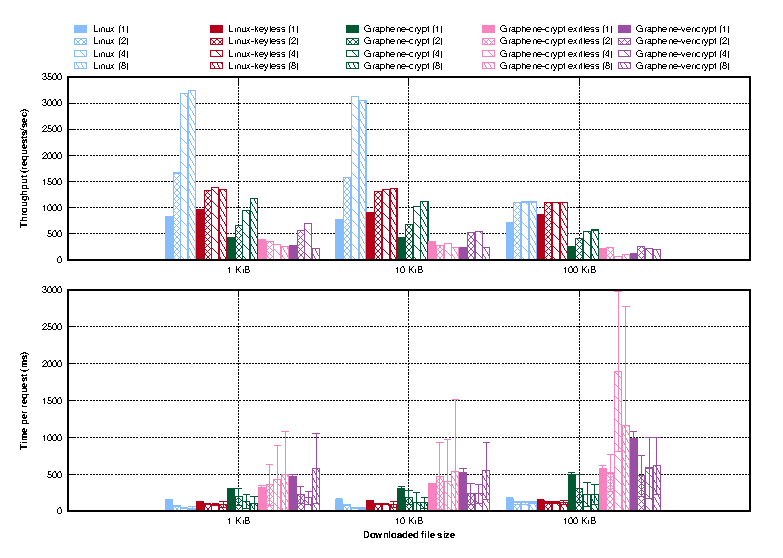
\includegraphics[width=\textwidth]{figs/macrobench-single-tenant-lat-throughput}
	%
	\caption{Throughput and latency for single tenant configurations.
    The legend indicates the number of NGINX worker processes.
    I include the standard deviation of the latencies as error bars.}
	%
	\vspace*{-4pt}
    \label{fig:macrobench-single-tenant-lat-throughput}
\end{figure}
